\chapter{Coulomb explosion imaging}\label{ch:CEI}

\vspace{-1.5 em}
\minitoc\hrule
\vspace{1.5 em}

\section{Physical principles}

% FOCUS ON THE HISTORY OF CEI IN DETERMINING GEOMETRIES
\section{Advances in molecular imaging}
The original CEI experiment is generally traced back to \citet{Vager89} in which the Coulomb explosion is initiated by passing a molecular beam through a thin foil. This is possibly because it was the first work claiming to report a molecular structure, as previous works utilizing CEI do exist, however they mainly report on energy and angle distributions. 

The laser makes its entrance surprisingly early 

There do exist other methods of initiating CEI, for example, single photons from a synchrotron source, x-ray pulses from a free-electron laser, or electron collision.

\subsection{Foil-forged images}
CEI was first performed by \citet{Vager89} whereby the Coulomb explosion was initiated by passing a molecular beam through a thin ($\sim30$ \AA) aluminum film at high velocities ($\sim0.02c$). Their work was motivated by the opportunity of imaging non-classical molecular structures that more popular methods were incapble of seeing. They were also the first to suggest that measuring the velocity (or momentum) vectors of each fragment would be provide all the information required to describe the molecule's structure. However, they do not perform any geometry reconstruction and report their fragment ion densities in a coordinate system defined by the asymptotic velocity of each particle, and claim that it is a direct measurement of the square of the multidimensional wave function of a many-body system.

\begin{figure}
  \centering
  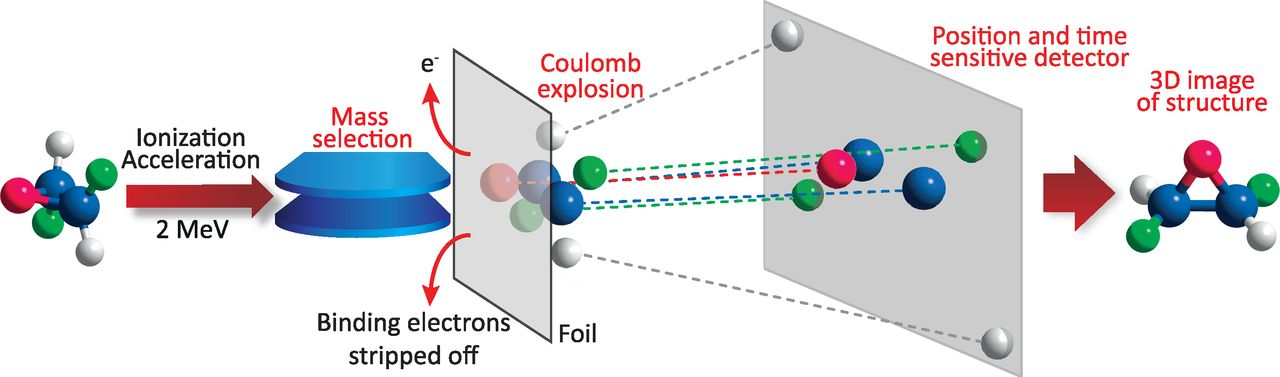
\includegraphics[width=\textwidth]{gfx/FoilExperiment}
  \caption[Schematic of a foil-induced Coulomb explosion imaging experiment.]
  {Schematic of a foil-induced Coulomb explosion imaging experiment. From \citet{Herwig13}. Reprinted with permission from AAAS.}
\end{figure}

One drawback of initiating Coulomb explosions using a thin foil is that a molecular beam must be prepared.

\subsection{CEI by highly charged ion impact}
\subsection{Laser-induced CEI}
\index{Coulomb explosion imaging!History}
\citet{Legare05structure,Legare05dynamics} was the first to use ultrashort laser pulses to induce Coulomb explosion and report on molecular structures and dynamics. To obtain the structures, they assume the explosion proceeds under a purely Coulombic potential and use optimization methods to make guesses at the structure that most accurately reproduces the observed data consistent with minimizing a least-squares objective function. Unfortunately they provide very minimal information regarding their methods and there is a complete lack of discussion acknowledging the shortcomings of this method\footnotemark. Using 8 fs laser pulses they report on the structure of D2O and SO2 \citep{Legare05structure}. They also claim to have imaged vibrating D2+ and dissociating SO22+ and SO23+ however they provide no more than a couple of dissociation frames and infer the transient D2+ bond length from kinetic energy release ratios as a function of pump-probe time delay \citep{Legare05dynamics}.

\footnotetext{The main shortcomings being degenerate solutions and the fact that they employ convex optimization methods to a problem that is not convex. It is not clear if they even knew about these issues.}

\index{Classical imaging formula}
\index{Coulomb explosion imaging!Classical imaging formula}
Surprisingly, an attempt was made to arrive at an analytical solution for calculating geometries from measured momentum data. \citet{Nagaya04} were able to derive a so-called classical imaging formulas giving the position wavefunction squared for the Coulomb explosion of a diatomic molecule and a linear triatomic molecule\footnotemark. They treat the cases of symmetric and asymmetric Coulomb explosion.

\footnotetext{They seem to have worked hard to find an analytical solution but their unsaid conclusion seems to be that it is an intractable problem and their group went silent on this problem.}

\citet{Gagnon08} reported the reconstruction of dichloromethane (CH2Cl2) using a home-made \footnotemark stochastic-based simulated annealing algorithm that globally optimizes the molecular spatial configuration. They discuss uncertainties but are only able to obtain the structure in five cases.

\footnotetext{There is nothing wrong with writing your own code here but nonconvex optimization algorithms are tricky to get right and the reliance should be on professional code.}

\index{Lookup table}
The best effort so far has probably been the one by \citet{Kunitski15} in which they use a lookup table approach to image the elusive Efimov state of the helium trimer.

\section{Outline of the experiment}

\subsection{Pump-probe Coulomb explosion imaging}
In pump-probe Coulomb explosion imaging (CEI) one ultrashort laser pulse is split into two pulses through the use an asymmetric beamsplitter. One of the pulses, the pump pulse, is usually much weaker than the other, the probe pulse. A time delay $\tau$ between the pulses is then created such that the pump pulse goes first and the probe pulse second. The job of the pump pulse will be to initiate some change in the molecule. One example could include an isomerization of the molecule. Thus the pump pulse ``pumps'' the molecule into some excited state. The job of the powerful probe pulse is to engulf the molecule in an intense enough laser field such that multiple electrons are stripped off of it. The molecule's individual atoms are left in a highly-charged state and begin to behave as individual point charges in a purely Coulombic potential. The entire process occurs in the presence of a constant electric field and so the positively-charged ions all accelerate upwards towards a time- and position-sensitive detector. Thus the probe pulse allows for the ``probing'' of the excited state.

\subsection{Femtosecond Multiple Pulse Length Spectroscopy}

\section{Experimental apparatus}

\section{Data analysis}

\subsection{Time and position measurement}
The position is then calculated using
\begin{equation}
x = \frac{Q_1 + Q_2}{Q_1 + Q_2 + Q_3 + Q_4} ,\quad
y = \frac{Q_1 + Q_3}{Q_1 + Q_2 + Q_3 + Q_4}
\end{equation}

\subsection{Calculating the atomic fragments' momenta}
The components of the three-dimensional momentum vector $\mathbf{p} = (p_x,p_y,p_z)$ for each atom are then calculated as

\begin{equation}\label{eq:CEImomenta}
p_x = \frac{m(x-x_0)}{t} ,\;
p_y = \frac{m(y-y_0)}{t} ,\;
p_z = \frac{qV}{2\ell} \left( \frac{t_0^2 - t^2}{t} \right)
\end{equation}
where $m$ is the atom's mass, $(x,y)$ is the location the atom collided with the MCP detector, and $(x_0,y_0)$ is the location that the Coulomb explosion originated. The location $(0,0)$ corresponds to the physical center of the MCP detector. $q$ is the net charge of the atom, $V$ is the value of constant electric potential the atom is subjected to, and $\ell$ is the distance from the location of the Coulomb explosion to the detector. $t$ is measured time of flight (between Coulomb explosion and detection) of the atom and 
\begin{equation}
t_0 = \sqrt{\frac{2d\ell}{V} \left( \frac{m}{q} \right)}
\end{equation}
is the atom's time of flight assuming no external forces act on it during its trip to the detector.

\subsection{Measurement uncertainty in the momenta}
For any relation $f = f(x_1, x_2, \dots, x_n)$, assuming independent variables, the absolute uncertainty in $f$, denoted $\Delta f$, may be calculated as
\begin{equation}
\Delta f = \sqrt{\sum_{i=1}^{n} \left( \frac{\partial f}{\partial x_i} \Delta x_i \right)^2}
\end{equation}
where $\Delta x_i$ is the uncertainty in the independent variable $x_i$.

Using this we may calculate the uncertainty in the measured momentum values, which will we different for each component. In our case, $p_x = p_x(m,x,x_0,t)$ and $p_y = p_y(m,y,y_0,t)$, however, the uncertainty in the atomic mass $m$ is orders of magnitude smaller than the uncertainty in the other variables and so we will ignore its effects. Thus we get that
\begin{subequations}
  \begin{align}
  (\Delta p_x)^2 &= \frac{\partial p_x}{\partial x}\Delta x + \frac{\partial p_x}{\partial x_0}\Delta x_0 + \frac{\partial p_x}{\partial t}\Delta t \\
  (\Delta p_y)^2 &= \frac{\partial p_y}{\partial y}\Delta y + \frac{\partial p_y}{\partial y_0}\Delta y_0 + \frac{\partial p_y}{\partial t}\Delta t
  \end{align}
\end{subequations}
where the partial derivatives can be calculated from \eqref{eq:CEImomenta} as
\begin{subequations}
  \begin{align}
  \frac{\partial p_x}{\partial x} = \frac{m}{t} &,\quad \frac{\partial p_x}{\partial x_0} = \frac{m}{t} ,\quad \frac{\partial p_x}{\partial t} = -m\frac{x-x_0}{t^2}\\
  \frac{\partial p_y}{\partial y} = \frac{m}{t} &,\quad \frac{\partial p_y}{\partial y_0} = \frac{m}{t} ,\quad \frac{\partial p_y}{\partial t} = -m\frac{y-y_0}{t^2}
  \end{align}
\end{subequations}
and so
\begin{subequations}
  \begin{align}
  \left( \frac{\Delta p_x}{p_x} \right)^2 &= \left( \frac{\Delta x}{x - x_0} \right)^2 + \left( \frac{\Delta x_0}{x - x_0} \right)^2 + \left( \frac{\Delta t}{t} \right)^2 \\
  \left( \frac{\Delta p_y}{p_y} \right)^2 &= \left( \frac{\Delta y}{y - y_0} \right)^2 + \left( \frac{\Delta y_0}{y - y_0} \right)^2 + \left( \frac{\Delta t}{t} \right)^2
  \end{align}
\end{subequations}

Repeating the process for $p_z = p_z(q,V,\ell,t_0,t)$ but ignoring the tiny uncertainties in $q$, $V$, and $\ell$, we get

\section{Computationally simulating a Coulomb explosion} \label{sec:simulating}
To simulate an explosion of a molecule containing $n$ atoms, we must solve the classical equations of motion for each ion right after the explosion. We choose to use Hamiltonian mechanics here to acquire a system of first-order differential equations which may be easily solved by numerical methods such as the ubiquitous fourth-order Runge-Kutta. Assuming a purely electromagnetic potential for each ion, the Hamiltonian of the molecular system is
\begin{equation}
\mathcal{H}(\mathbf{r}_i, \mathbf{p}_i, t) = \sum_{i=1}^n \frac{\mathbf{p}_i^2}{2m_i} + \frac{1}{4\pi\epsilon_0}\sum_{\substack{\lbrace i,j\rbrace\\ i \ne j}} \frac{q_iq_j}{|\mathbf{r}_i-\mathbf{r}_j|}
\end{equation}
where $i,j \in \lbrace 1,2,\dots, n \rbrace$ and so the second summation is over all $i,j$ pairs where $i \ne j$. Calculating Hamilton's equations for the system, we get
\begin{subequations}
  \begin{align}
  \frac{d\mathbf{r}_i}{dt} &= \frac{\partial \mathcal{H}}{\partial \mathbf{p}_i} = \frac{\mathbf{p}_i}{m_i} \\
  \frac{d\mathbf{p}_i}{dt} &= \frac{\partial \mathcal{H}}{\partial \mathbf{r}_i} = \frac{1}{4\pi\epsilon_0}\sum_{j, \; j \ne i} \frac{\mathbf{r}_i - \mathbf{r}_j}{|\mathbf{r}_i - \mathbf{r}_j|^3}
  \end{align}
\end{subequations}
where $i$ is held fixed over the second summation. With appropriate initial conditions this system of $6n$ scalar first-order ordinary differential equations may be easily solved using, for example, the classical fourth-order Runge-Kutta method for numerically solving ordinary differential equations. The atoms are assumed to be at rest so that $\mathbf{p}_i(t=0) = 0$, while the initial positions, $\mathbf{r}_i(t=0) = 0$, are chosen to correspond to the molecular geometry. \footnote{Discuss the validity of the at rest assumption.}

One way to think of the problem being tackled in this thesis is: which initial geometry $\mathbf{r}_i(t=0) = 0$ results in the momentum values measured at the detector? The atoms are far enough apart after just a few nanoseconds that by the time they arrive at the detector, they feel almost no forces due to each other and their momenta attain asymptotic values which we can denote $\mathbf{p}_i(t\rightarrow\infty)$.

\section{Conventions for geometries and momenta}

\subsection{Describing molecular geometries by a Z-matrix}

\subsection{A homemade convention to describe momentum vectors}
